\chapter{Introduction}


Today's Internet is an ``eyeball economy'' dominated by applications such 
as video streaming (e.g., video traffic was 70\% of all consumer Internet 
traffic in 2015 and is forecasted to be 82\% of consumer Internet traffic by 
2020~\cite{cisco-forecast-2015}) and VoIP (e.g., Skype users spend over 
2 billion minutes talking to each other every day~\cite{skype-2-billion-minutes}). 
With most application providers relying on more user engagement to generate 
revenues, maintaining high user-perceived {\em QoE} (Quality of Experience) 
has become crucial to ensure high user engagement and support the 
existing revenue models~\cite{sigcomm13athula}.
For instance, recent research shows even one short video buffering 
interruption leads to 39\% less time spent watching videos and can 
causes significant  revenue losses for ad-based video sites. 
Suboptimal QoE is damaging to subscription-based 
service providers as well. For instance, my work with Microsoft shows 
most Skype  users give low rating when experiencing an average of 
1.2\% packet loss~\cite{via}.

Therefore, understanding and improving QoE of Internet applications 
has recently become a focus of intense academic and industry efforts. 
The trend is exemplified by the growing number of 
publications (e.g.,~\cite{sigcomm13athula,sigcomm12,
wang2014speedy,sigcomm11,eona,krishnan2013video}), workshops 
(e.g.,~\cite{workshop-wmust,workshop-fhmn,workshop-qoe}), 
and start-ups (e.g., \cite{conviva,artizanetworks}) focusing on QoE optimization 
in diverse applications such as video streaming, Internet telephony, mobile 
apps and web services.

%\begin{itemize}
%\item Overview of Internet applications: video streaming and internet telephony
%\item Re-architect the core -- high deployment cost
%\item Per-edge adaptation -- too narrow view
%\end{itemize}

%\section{Ensuring High QoE is Challenging}

\jc{need to shrink it} While there have been intense efforts towards improving Internet 
QoE over the past decades, existing approaches fail to deliver the 
QoE needed by today's applications. 
Figure~\ref{fig:intro:badqoe} presents the QoE distribution and the 
prevalence of bad QoE in video streaming and Internet telephony, 
two of the most popular applications today.
Figure~\ref{subfig:intro-badqoe-video-buffering} shows that among 
over 300 million video sessions from 376 content 
providers, while most of them do not experience re-buffering 
(video stalls), 12\% video sessions spent over 1\% of time in re-buffering,
and 5\% sessions waste even 10\% of the view time in 
re-buffering~\cite{jiang2013shedding}, which could cause significant 
loss on average view time and number of views, especially for 
live content~\cite{sigcomm11}. 
Note that these results are based on study of US-based content 
providers whose viewers have good broadband penetration, 
and QoE is much worse in less developed regions.
Similarly, Figure~\ref{subfig:intro-badqoe-skype-lossrate} shows that 
among 430 million Skype calls that were not relayed by an intermediate
machine, 17\% calls had experience over 1.2\% packet loss in the 
duration of a call~\cite{via}. 
To put the numbers into perspective, user studies on QoE of VoIP have 
shown that over 1\% of packet loss could cause frustrating experience
of VoIP calls~\cite{itu,cisco-voip}.
Note that the packet loss rate is on the average values over the
call's duration during which there may be transient spikes
(e.g., loss burst) in bad performance.


\begin{figure}[t!]
\captionsetup[subfigure]{justification=centering,farskip=-1pt,captionskip=5pt}
\centering
%\hspace{-0.5cm}
\subfloat[Video streaming]
{
        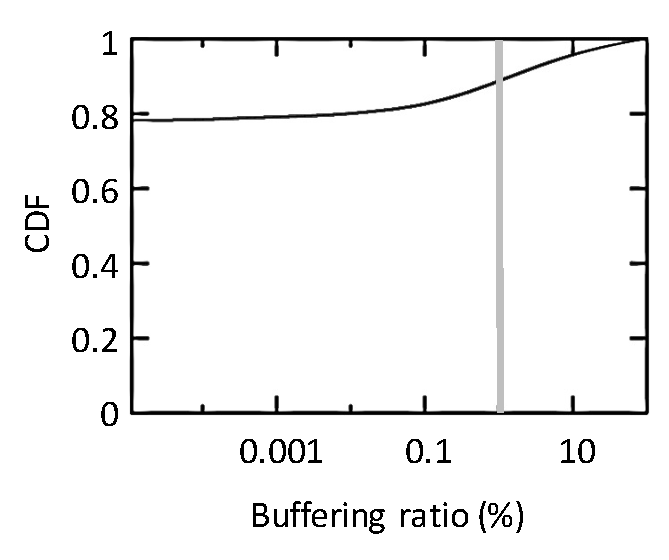
\includegraphics[width=0.35\textwidth]{figures/intro-badqoe-video-buffering.pdf}
        \label{subfig:intro-badqoe-video-buffering}
}
%\hspace{-0.1cm}
\subfloat[Internet telephony]
{
        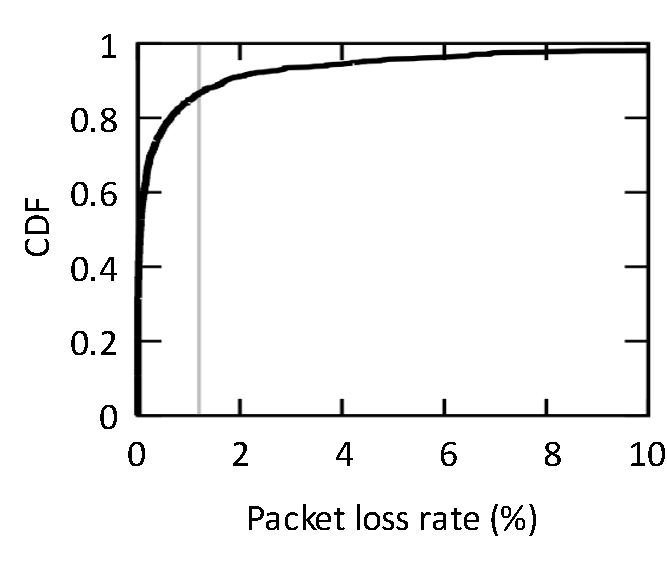
\includegraphics[width=0.35\textwidth]{figures/intro-badqoe-skype-lossrate.pdf}
        \label{subfig:intro-badqoe-skype-lossrate}
}
%\vspace{-0.2cm}
\caption{QoE distributions of video streaming and Internet telephony. 
The figures shows that a substantial fraction of video sessions (12\%) 
and VoIP calls (17\%) suffer from bad QoE (over 1\% buffering ratio 
and 1.2\% packet loss rate, respectively).
Buffering ratio is the fraction of video session duration spent in 
re-buffering (video stalls), and is one of the key metrics of video 
streaming QoE. 
Packet loss rate is calculated over the call's duration, and is shown to 
have significant impact on VoIP user experience.}
%\vspace{-0.1cm}
\label{fig:intro:badqoe}
\end{figure}

To see the reason that prior research has failed to deliver desirable 
QoE in a substantial fraction of cases, one has to understand
their fundamental limitations. 
Classic networking approaches to Internet QoE optimization fall
into two broad categories. 

\begin{itemize}
\item Research in the first category seeks to {\em re-architect the network core}, 
so that ISPs can provide
better or even guaranteed quality of service (i.e., QoS). 
Though this direction has led to many influential projects 
(e.g.,~\cite{demers1989analysis,stoica1998core,tennenhouse2002towards}),
it is hard to make any significant changes to the network core in the real world. 
Besides, these network-core devices, such as routers or switches have 
limited visibility into applications running in the client devices, so they cannot
directly optimize for application-level QoE.

\item The second category, {\em endpoint adaptation}, seeks to use
intelligent logic in individual client-side devices to  utilize the existing 
network resource.
This approach is pervasively used in many protocols from 
application layer (e.g., video bitrate adaptation~\cite{dash}),
transport layer (e.g.,congestion control~\cite{jacobson1988congestion}),
down to link layer (e.g.,wireless rate adaptation~\cite{holland2001rate}).
Arguably more deployable than changing the network core, the approach 
of endpoint adaptation suffer from the key limitation that
it can only use the local information visible to individual endpoint to
{\em react} to dynamic network conditions or resource availability.
We observe a growing decision space of potential control decisions 
to optimize application quality.
Consequently, trial-and-error strategies driven by single-session feedback are
fundamentally inefficient and slow in exploring the decision space and reacting to
changes. For instance, it takes a video player several chunks (roughly 10s of
seconds) to converge to an optimal combination of CDN and bitrate~\cite{dda-report}.
%Due to this limited knowledge of network conditions, it is difficult for 
%the endpoint adaptation to cope with the {\em growing decision space} 
%of potential control decisions to optimize application quality.

%of endpoint adaptation suffer from two limitations: 
%(1) it can only use the information visible to individual endpoint to react to dynamic network 
%conditions or resource availability,
%and (2) it typically uses manually designed strategies. 
%These two features inherently mismatch two recent trends of Internet applications
%First, we observe a {\em growing decision
%space} of potential control decisions to optimize application quality.
%Consequently, trial-and-error strategies driven by single-session feedback are
%fundamentally inefficient and slow in exploring the decision space and reacting to
%changes. For instance, it takes a video player several chunks (roughly 10s of
%seconds) to converge to an optimal combination of CDN and bitrate~\cite{dda-report}.
%Second,  we see an {\em increasing heterogeneity} in operating conditions, each requiring
%different control logic and parameters.  For instance, TCP parameters such
%as initial congestion window and AIMD parameters could be tweaked to work
%better in different operating conditions~\cite{remy,googleinitwindow}.
\end{itemize}


\section{Contributions}

The key contribution of this thesis is to demonstrate the feasibility of a new 
{\em data-driven approach}:
{\em one can significantly improve QoE of Internet applications by leveraging
real-time, global view of QoE of millions of endpoints to drive the
adaptation of individual endpoints.}
My research makes this contribution through elaborating key technical 
challenges of the data-driven approach, addressing these challenges by
novel algorithms and system architectures that integrate domain-specific 
insights with machine learning,
and using large-scale datasets and pilot deployments to demonstrate
the real-world QoE improvement brought by this data-driven approach.

At a high level, the new data-driven approach envisages a logically centralized 
{\em controller}, which collects QoE observed by many application clients, 
uses the data to maintain a real-time, global view of network conditions,
and uses the data to make real-time decisions
regarding configurations or adaptations of clients, flows, or application sessions.
A good case in point of this architecture is that a video content provider can 
collect session-level QoE measurements (e.g., buffering events) from 
the video players running on its viewers, and use these measurements of 
history and concurrent video sessions to predict for any new session the best
bitrate and CDN selection~\cite{c3}.

\begin{figure}[t!]
\captionsetup[subfigure]{justification=centering,farskip=-1pt,captionskip=5pt}
\centering
\hspace{-0.5cm}
\subfloat[Classic approaches.]
{
        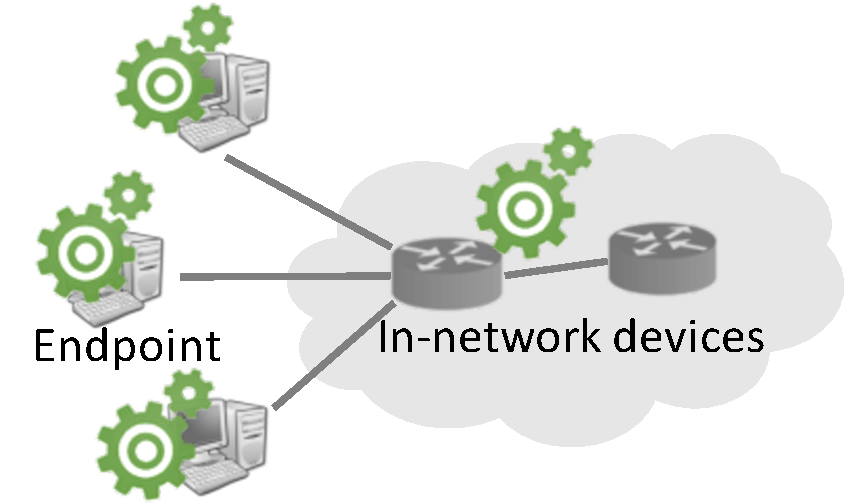
\includegraphics[width=0.4\textwidth]{figures/intro-classic.pdf}
        \label{subfig:problem-of-epsilon:change}
}
%\hspace{-0.1cm}
\subfloat[The new data-driven approach.]
{
        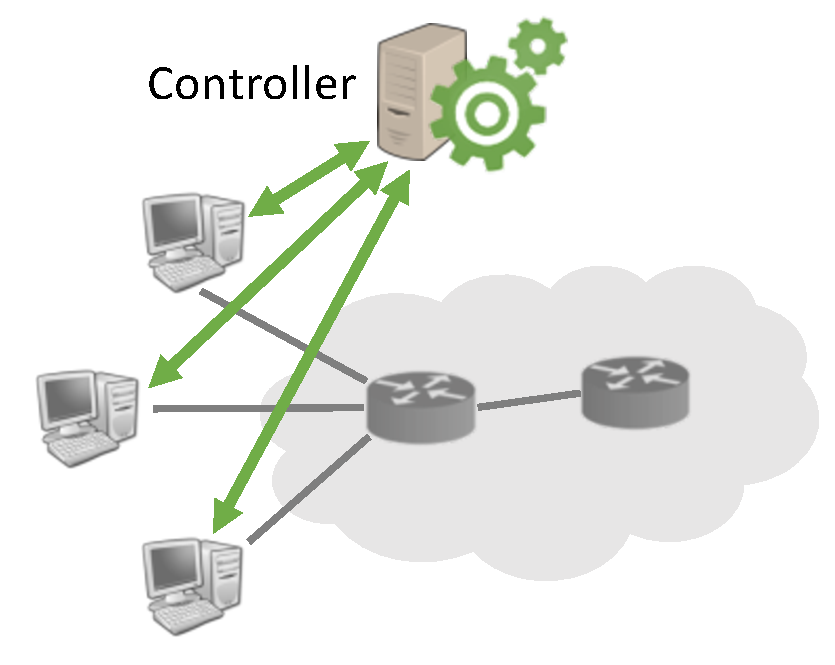
\includegraphics[width=0.4\textwidth]{figures/intro-ddn.pdf}
        \label{subfig:problem-of-slow:load}
}
\vspace{-0.2cm}
\caption{Contrasting the new data-driven approach with classic approaches. 
The key different lies in where to implement the functionality of QoE optimization (symbolized by the gears): the classic approaches implement 
it in the network core or individual endpoint, whereas the new data-driven approach implements 
it in the controller that maintains a real-time global view of QoE of millions of endpoints.}
\vspace{-0.1cm}
\label{fig:intro:contrast}
\end{figure}

Figure~\ref{fig:intro:contrast} highlights the contrast between
the data-driven approach and classic ones.
The key different lies in {\em where to implement the functionality of QoE 
optimization}: 
the classic approaches implement it in the network core or individual endpoint, 
whereas the new data-driven approach implements it in the controller 
that maintains a real-time global view of QoE of millions of endpoints.
Moving the QoE optimization to the controller offers
inherent advantages over both categories of classic approaches.
On one hand, making more intelligent adaptation at endpoints, 
even when an overlay system of the endpoints is needed, 
is more flexible and deployable than re-architecting the network core, as 
demonstrated by prior work (e.g.,~\cite{chu2002case}).
On the other hand, using the QoE measurements from multiple endpoints 
addresses the limitation of endpoint adaptation -- instead of using
reacting to dynamic network conditions with a local view, one can {\em predict} 
the QoE a client would experience if the client uses certain decisions.

The new data-driven approach is also fortuitously aligned with a confluence of 
recent  ``technology pulls''. 
First, we observe that many application providers today have widely deployed client-side 
instrumentation to collect massive real-time in-situ performance data  (e.g.,~\cite{sigcomm11,via,imc12akamai,artizanetworks}). 
Second, the emergence of large-scale analytics systems provides the ability to extract insights efficiently from large corpses 
of data (e.g.,~\cite{spark}) and from stream of updates (e.g.,~\cite{zaharia2013discretized}). 
Such ability enables optimal decision making based on real-time data-driven 
predictions~\cite{velox-cidr}.
Finally, control plane platforms have been built in many service providers, such as content providers~\cite{c3} and CDNs~\cite{mukerjee2015practical}.

%\begin{itemize}
%\item {\em More measurement data in networking:}
%Many application providers today have widely deployed client-side 
%instrumentation to collect real-time performance data. 
%
%\item {\em ``Big data'' platforms finally a reality:}
%The emergence of large-scale analytics systems provides the ability to extract insights efficiently from large corpses 
%of data (e.g.,~\cite{spark}) and from stream of updates (e.g.,~\cite{dstream}). 
%Such ability enables optimal decision making based on real-time data-driven 
%predictions~\cite{velox}.
%
%\item {\em Wide use of control platforms:}
%Control plane platforms have been built by many individual subsystems (e.g., ISPs, video service providers and CDNs).
%
%\end{itemize}


%To take a concrete example, let’s think about Netflix player. 
%Traditionally, it takes a Netflix video player tens of seconds to converge to a good 
%quality, while in the new data-driven approach, Netflix can achieve much better 
%quality by using real-time quality measurement from many video players to directly 
%predict the best configuration for individual Netflix players.


%\subsection{Opportunities}

%\mypara{Opportunities of data-driven networking} 
%The data-driven approach is fortuitously aligned with several recent technology trends. Specifically, 
%
%\begin{itemize}
%\item {\em More measurement data in networking:}
%Many application providers today have widely deployed client-side 
%instrumentation to collect real-time performance data. \jc{examples}
%
%\item {\em ``Big data'' platforms finally a reality:}
%The emergence of large-scale analytics systems provides the ability to extract insights efficiently from large corpses 
%of data (e.g.,~\cite{spark}) and from stream of updates (e.g.,~\cite{dstream}). 
%Such ability enables optimal decision making based on real-time data-driven 
%predictions~\cite{velox}. \jc{examples}
%
%\item {\em Wide use of control platforms:}
%Control plane platforms have been built by many individual subsystems (e.g., ISPs, video service providers and CDNs). \jc{examples}
%
%\end{itemize}

\mypara{Challenges}
While the new data-driven approach enjoys several advantages over 
classic approaches and could achieve much better QoE for Internet 
applications, it is still challenging to unleash its full potential.
This thesis focuses on two fundamental challenges unique to applying 
data-driven approaches in networking:

\begin{enumerate}

\item 
%{\em The need for expressive models} to capture complex factors affecting QoE. 
First, the controller needs to extract actionable insights, such as a 
predictive model to predict QoE based on client-side features, from 
the data stream of QoE measurements. 
Consequently, we need an {\em expressive models} to capture complex 
factors affecting QoE. 

\item 
%{\em The need for scalable platforms} to make real-time decisions with fresh data from geo-distributed clients.
Second, the controller needs to turn the actionable insights into 
real-time control decisions to be executed by geo-distributed clients. 
This requires a {\em scalable platforms} to make real-time decisions 
with fresh data from geo-distributed clients.

\end{enumerate}

\mypara{Key insights and ideas}
This thesis addresses these challenges in practice by integrating 
several domain-specific insights in networked applications with 
machine learning algorithms and systems, and achieves better QoE 
than using off-the-shelf machine learning solutions. 
The unifying theme underlying these domain-specific insights is 
that there exists some {\em persistent structures} -- 
these structures help identify network sessions with similar 
QoE-determining factors, and that such structures tend to be 
persistent on timescales of tens of minutes.
To see concrete example of a persistent structure, let us consider 
a group of network flows bottlenecked by a congested link.
The throughput of these flows may vary over time, but the fact
that these flows are bottlenecked by this congested link remains true 
for the whole duration of the congestion event.
In this example, the structural property is the congested link, and 
it is more persistent than the Internet performance.

The insight of persistent structures enable us to address the 
aforementioned challenges.
At a high level, these domain-specific structures 
allow us to build expressive models that can identify network 
sessions with similar QoE-determining factors.
Meanwhile, because these structures are persistent, we can 
build scalable systems by decoupling the offline structure-learning 
process and the real-time decision making process.



\section{Summary of Results}

Based on the insight of persistent structures, I developed novel algorithms 
and end-to-end systems, and deployed them in real world to 
improve QoE for two applications: Internet video streaming, 
and internet telephony. 
These improvements can lead to significant benefit for the application providers.





\paragraph{CFA: Improving QoE via Expressive Prediction Models.}
%problem
Delivering high QoE is crucial to the success of today's subscription-/ad-based business models for Internet video.
There is substantial room for improving video QoE by dynamically selecting the optimal CDN (Content Delivery Network) and bitrate based on a real-time global view of network conditions~\cite{sigcomm-case,conext-shedding}.
The key to realizing this promise is a {\em prediction oracle} that can accurately predict the quality of a video client if it uses a certain CDN and bitrate.
%challenge
The challenge is that this prediction system must be (a) expressive enough to capture complex relations between video quality and observed session features, and (b) capable of updating quality predictions in near real time.
We used several off-the-shelf machine learning techniques, such as random forests and SVM, but found they did not produce expected QoE improvements, because the long-term historical data is too coarse grained for these algorithms to capture the dynamics of video quality, while the short-term historical data is not sufficient for the algorithms to learn complex relations between video quality and observed session features.
%these algorithms fail to capture the quality variability when trained with long-term history data, and they fail to identify the complex prediction models when trained with short-term history data.
%Unfortunately, several seemingly natural solutions (e.g., simple machine learning approaches and network models) fail on one or both fronts.
%insight
My solution, CFA~\cite{cfa}, leverages the domain-specific insight of {\em persistent critical features}; each video session has a small set of critical features that ultimately determines its video quality, and these critical features change much more slowly than video quality~\cite{conext-shedding}. 
%I present the design and implementation of CFA~\cite{cfa} to address these challenges. 
%CFA is driven by the domain-specific insight of {\em persistent critical features}, that each video session has a subset of critical features that ultimately determines its video quality, and these critical features tend to be persistent on timescales of tens of minutes~\cite{conext-shedding}. 
%solution
This insight enables us to learn complex prediction models from long-term historical data (thus expressing complex relations between video quality and session features), and update the models by short-term historical data in near real time (thus capturing quality fluctuation as well).
%Therefore, CFA can predict video quality more accurately than many machine learning algorithms, though CFA may not be as good in other prediction tasks.
%result
A real-world pilot deployment shows that CFA leads to non-trivial improvements in video quality, e.g., 32\% less buffering time than industry-standard algorithms.
Our conversation with domain experts confirmed that these improvements are significant for content providers and can potentially translate into substantial benefits in revenues.
An end-to-end implementation of CFA has been deployed and used by Conviva, a company that offers video quality optimization services to many premium content providers. 

The insight of persistent critical features turns out to be more general; e.g., I have also applied the same insight to accurate prediction of TCP throughput~\cite{cs2p}, which leads to 11\% higher video bitrate than state-of-the-art adaptive bitrate players (e.g., Netflix players) with no extra buffering.


%\mypara{\underline{\smash{Real-Time Exploration and Exploitation At Scale.}}}
\paragraph{Pytheas: Improving QoE via Exploration and Exploitation at Scale.}
%\mypara{Real-Time Exploration and Exploitation at Scale:}
%problem
While formulating data-driven QoE optimization as a prediction problem has shown promising QoE improvement (e.g., CFA), 
it is necessarily incomplete, as 
it suffers from many known biases such as incomplete visibility, and cannot respond to sudden changes such as flash crowds.
Drawing a parallel from machine learning (e.g., ad recommendation), I argued that data-driven QoE optimization should instead be cast as a {\em real-time exploration and exploitation} process. % rather than as a prediction problem. 
Measurement collection (exploration) could be informed by decision making (exploitation) to explore the decisions with less data, thus addressing the shortcomings of the prediction-based formulation.
This new formulation is complementary to CFA, since CFA's prediction model can be reused to capture similarities among clients.
%challenge
While many exploration-and-exploitation algorithms are available, enabling these algorithms in networking introduces an architectural challenge: we need a {\em scalable control platform} to update decisions with fresh global data from clients, despite data coming from a variety of geo-distributed front-end clusters, each with only a partial view of the clients.
%The key challenge of real-time exploration and exploitation in networking is how to update decisions in real-time for millions of geo-distributed clients using their fresh measurement data.
%insight
A baseline approach is to run control logic in a single back-end cluster with global data from front-end clusters, but this approach leads to non-trivial staleness of the global data and suboptimal decisions.
I take an alternative approach; the control logic is run by geo-distributed front-end clusters which have fresh data, rather than the back-end cluster.
The intuition is that the clients that exhibit similar QoE behavior will have similar network-level features (e.g., same IP prefix), and thus their fresh data will likely be collected by the same front-end cluster.
%While the challenge might be intractable in a general setting, it
%I address the challenge by the insight that network application sessions sharing the same {\em network- and application-level features} intuitively exhibit similar QoE behavior across different possible decisions.
%solution
Inspired by this insight, {Pytheas}~\cite{pytheas} uses the concept of {\em group-based exploration and exploitation}, which 
%The key idea is to decompose the global exploration and exploitation process of all clients into processes within groups of similar clients and run these per-group processes in geo-distributed front-end clusters which are close to clients and have their fresh data.
%The key idea is to decompose the global exploration and exploitation process into subprocesses of similar clients, and run each subprocess by the front-end cluster that is close to its clients and has their fresh data.
decomposes the global exploration and exploitation process into subprocesses, each controlling a group of similar clients and running in the front-end cluster that has these clients' fresh data.
%with both client-closeness and data-freshness.
%result
Using an end-to-end implementation in CloudLab, I show that compared to a state-of-the-art prediction-based system, Pytheas improves the average video QoE by up to 31\% and the 90th percentile QoE by 78\%.
Pytheas is an open source project that enables application providers to deploy the proposed architecture at scale within their existing infrastructure. 

 
%\mypara{\underline{\smash{Reducing Large Decision Space.}}} 
\paragraph{VIA: Improving QoE in the Face of Large Decision Spaces.} 
%\mypara{Reducing Large Decision Space:}
%problem
In the first large-scale study on Internet telephony quality, I found that a substantial fraction of Skype calls suffer from poor network performance, and that there is much room for improving Skype quality by routing each call through the optimal relay clusters in Microsoft's cloud.
%challenge
However, identifying a close-to-optimal relay in practice is very challenging, due to the sheer number of possible relay paths (in hundreds) and their dynamic performance (which could change on timescales of minutes). 
Neither prediction-based methods (e.g., CFA) nor those based on exploration and exploitation (e.g., Pytheas) suffice to handle such a large decision space.
%insight
The key insight to address this challenge is that, for each pair of caller ISP and callee ISP, there is a {\em small and stable subset} of relays that almost always contains the best relay. 
This insight has two implications: (1) because this subset of relays is stable, it can be learned from history; and (2) because this subset has only a few relays (less than five), it can be explored efficiently even with limited data.
%the large decision space can be narrowed down to a {\em small subset} of relays that almost always contains the best relay, and such pruning can be learned from the historical data, because this set of most promising relays tends to be {\em persistent}.
%solution
Inspired by these intuitions, I developed {VIA}~\cite{via}, a relay selection system that achieved close-to-optimal quality using the concept of {\em guided exploration}. The idea is to learn a small set of promising relays for each ISP pair based on long-term (e.g., daily) historical data, and explore these relays using most calls in real time.
%result
Trace-driven analysis and a small-scale deployment shows that VIA cuts the incidence of poor network conditions for calls by 45\% (and for some countries and ISPs by over 80\%) compared to today's Skype quality.
VIA has been used in Microsoft internal deployment with real Skype users, and is in the process of being fully deployed. 
VIA was also used by Microsoft to identify the countries and ISPs where Skype quality can benefit the most if relaying services are deployed.
%VIA is also used to identify the countries and ISPs where Skype quality can benefit the most from Microsoft relaying services.


The key promise here is that by using more data, networking research can 
benefit from the ``unreasonable effectiveness of data''~\cite{google-data}, 
which has transformed the landscape of many research fields 
(such as natural language processing and computer vision) in the recent years.
Inspired by these recent successes of data-driven approaches, 
I believe networking should be no difference. 
